\section{Introduction}

Many multi-processor systems use the MESI protocol for cache coherence \cite{Primer_on_Memory_Consistency}, which provides sequential consistency for any data race-free program. However, the cache coherence protocol might make redundant or indirect requests because it does not know about the program structure.

For example, suppose a program directs each processor to compute one layer of a neural net in a pipelined fashion (see \cref{fig:pipelined_net}). Processor \(i\) needs to send its activation's to Processor \(i+1\) so that Processor \(i+1\) can compute the next layer of activations. In traditional MESI system, Processor \(i\) would store data to its cache, in `exclusive' state. Then Processor \(i+1\) would attempt to load the data, miss in its cache, go to the bus, ask Processor \(i\) for data, downgrading \(i\)'s copy to `shared' state.

\begin{figure}[h]
  \centering
  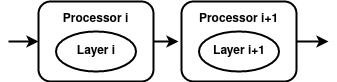
\includegraphics[width=0.375\textwidth]{pipelined_parallelism.png}
  \caption{The dataflow graph of pipelined neural net inference}
  \Description{Dataflow graph where Processor \(i\) computes layer \(i\) and sends activations to Processor \(i+1\).}
  \label{fig:pipelined_net}
\end{figure}

An optimization is available: The compiler could prove that Processor \(i+1\) is the consumer of the activations written by Processor \(i\), so it could instruct Processor \(i\) to send its data directly to the cache of Processor \(i+1\), bypassing the Last-Level Cache (LLC) \cite{DeNovo}.  Streaming programs spend a substantial portion of their time and energy in the Network on Chip (NoC), so optimizations like this save power and time \cite{dynamic_cache_coherence}.

Many of these coherence optimizations are only beneficial in specific cases, so the architecture needs to dynamically select the best coherence optimization for the given memory-locations based on the access pattern while maintaining correctness. The architecture only knows about historical access patterns and does not know what the other processors in the system are doing, so it is difficult for the architecture to select a coherence optimization by itself. The compiler can form an expectation of future access patterns and could know what other processors in the system are doing, so it should inform the architecture what coherence optimization to use for specific memory-locations.

Our contribution is a compiler-pass which analyzes the access pattern of the given program to identify certain opportunities for coherence optimization. We hope future work will build on this pass to support more kinds of coherence optimizations and develop a better cost-model. Our implementation leverages the HPVM compiler Intermediate Representation (IR) \cite{HPVM} and emits coherence optimizations for the Spandex Cache Coherence protocol \cite{Spandex}.